\documentclass[11pt]{article}
\usepackage[utf8]{inputenc}
\usepackage{amsmath}
\usepackage{amsfonts}
\usepackage{amssymb}
\usepackage{graphicx}
\usepackage[super]{nth}
\usepackage{amsthm}
\usepackage{bm}
\newtheorem{theorem}{Theorem}
\newtheorem{objective}{Objective}
\newtheorem{model}{Model}
\usepackage{xcolor}
\definecolor{light-gray}{gray}{0.95}
\newcommand{\code}[1]{\colorbox{light-gray}{\texttt{#1}}}
\usepackage{listings}
\usepackage{placeins}

\usepackage[authoryear]{natbib}


\makeatletter
\renewcommand{\maketitle}{
\begin{center}

\pagestyle{empty}

{\LARGE \bf \@title\par}
\vspace{1cm}

{\Large Marcel Gietzmann-Sanders, Michael Courtney, Andrew Seitz, Curry Cunningham}\\[1cm]

University of Alaska Fairbanks


\end{center}
}\makeatother


\title{A Framework for Studying Animal Behavior Using Deep Learning}

\date{2024}
\setcounter{tocdepth}{2}
\begin{document}
\maketitle


\begin{center}
This study explores using deep learning to build Individual-Based Models (IBMs). Using Chinook salmon (\textit{Oncorhynchus tshawytscha}) PSAT data as a case study, we introduce a methodology that leverages deep learning to transform the construction of IBMs into a systematic tool for investigating behaviors and their covariates. By employing a "log-odds model" to reduce dimensionality, this approach positions modeling as a central driver of discovery, enabling efficient hypothesis testing and iterative refinement.
\end{center}



\section*{Introduction}

Individual-Based Models (IBMs) have emerged as a critical tool for studying ecological systems, particularly for capturing the nuanced behaviors and interactions of individual organisms within their environments \citep{grimm}. With them, investigators can propose hypotheses on how fish behave and then test those hypotheses against actual individual behaviors as observed in the wild.

However, current methods for building IBMs are largely bespoke, tailored to specific systems or questions, and often require extensive manual development and calibration \citep{grimm}. This lack of standardization poses significant challenges to their broader adoption as a foundational methodology for studying behavior \citep{grimm}. Each model requires unique assumptions, data integrations, and computational workflows, making it difficult to generalize findings across studies or species. 

Machine learning offers a way to at least partially address the bespoke nature of traditional Individual-Based Models (IBMs). By framing individual behaviors as probabilistic decisions among consecutive sets of choices each described by a series of features, machine learning can be invoked to largely automate the process of building the decision "engine" behind IBM's. Machine learning excels at identifying patterns in high-dimensional data, enabling models to dynamically incorporate a wide range of environmental and behavioral covariates without requiring custom coding for every new hypothesis. Furthermore, by providing a consistent framing, the same systems and tools can be used across a variety of different problems. 

Beyond offering a common framework, reducing the time required to build IBMs allows investigators to focus on using the modeling process to quickly test hypotheses and identify areas of uncertainty early in their studies. This efficiency enhances the utility of IBMs, making them an even more powerful tool for advancing the understanding of complex behaviors.

In this study we demonstrate how integrating machine learning with Individual-Based Models (IBMs) provides a standardized, efficient approach for testing hypotheses and refining models, enabling rapid exploration of behavior and uncertainty.

\section*{Framing}

The methodology centers on a two-stage cycle of discovery: (1) testing hypotheses about covariates that are believed to predict behaviors and (2) using the results to generate new hypotheses.

In the first stage, we model behaviors as decisions made from a set of choices, each associated with hypothesized covariates. Then, using deep learning, we build a predictive model to evaluate the likelihood of these selections based on the covariates.

In the second stage, we evaluate how the model shifts the likelihood of specific individuals or decision groups relative to baseline models. Improved performance reveals where the covariates more effectively predict behavior, while underperformance indicates missing covariates. This focus on areas of "greatest possible effect" provides case studies for generating new hypotheses, enabling iterative refinement of the process.

The keystone of this entire process is having a clear, quick means of producing deep learning models from our framing of decisions, choices, and covariates, an issue which we turn to next. 

\section*{Theory}

Standard probabilistic deep learning networks are typically framed as a classification problem, using categorical cross-entropy as the loss function \citep{durr}. Each output neuron represents a potential choice, with the model predicting the probability of each choice being correct based on this loss formulation. For these choices, we provide the network with features encapsulating the relevant information. Training is then comprised of providing a series such decisions. 

However, this formulation introduces a critical challenge: if there are $N$ features per choice and $M$ potential choices, the overall dimensionality of the input space becomes $N \cdot M$. Adding even a single feature increases the dimensionality by $M$ not just 1.

This growth poses a significant challenge due to the "curse of dimensionality", where the amount of data required to effectively train models can grow exponentially with the dimensionality of the input space \citep{curse}.

\subsection*{Log-Odds Modeling}

To address this issue, we propose an alternative framing. Instead of predicting the probabilities directly, we predict the log-odds $\phi_m$ for each choice and calculate the probability $p_m$ using the softmax function:

$$p_m = \frac{e^{\phi_m}}{\sum_{m=1}^{M}e^{\phi_m}}$$

This approach reduces the feature space dimensionality to $N$ and effectively increases the number of training examples by a factor of $M$.

We can implement this log-odds model using standard probabilistic deep learning techniques by replicating the "log-odds model" weights across all $M$ choices. The outputs are fed into a softmax layer with $M$ units, where the layer's weights are set to the identity matrix and biases are set to zero. Using categorical cross-entropy as the loss function ensures compatibility with standard probabilistic deep learning while enabling us to train the log-odds weights and significantly reduce the problem's dimensionality.

\subsection*{Contrast Sampling}

As $M$ grows large, a practical issue arises: for each training example, most instances of the internal log-odds model would ideally report very low log-odds, resulting in low probabilities. Ideally, only one choice should produce $p_m=1$. This is analogous to a class imbalance problem, where the model becomes prone to predicting the most common class.

To address this, we balance the training data. Instead of presenting the model with full decisions containing all $M$ choices, we create training pairs, or contrasts, where each pair consists of one selected choice and one unselected choice. This approach is valid because the log-odds model focuses on the relative likelihood of choices, making the number of choices considered at any one time irrelevant.

The primary risk in using contrasts is introducing bias by disproportionately sampling certain combinations of choices. To mitigate this, we randomly sample pairs from each decision, ensure an equal number of contrasts per decision, and an equal number of decisions per individual. This preserves the balance across the training data and avoids skewing the model's predictions.

\subsection*{Alternative Approaches to Reducing Dimensionality}
There are other strategies for reducing the dimensionality of one's data. One straightforward method is to limit the choices available. For instance if making decisions among a set of directions, one could reduce the precision of the angles allowed. While this approach reduces the model's specificity, it significantly simplifies the dimensionality of the problem.

The methodology proposed here, however, achieves dimensionality reduction without sacrificing specificity. That said, there are scenarios where some choices are unlikely to be relevant. In such cases, dimensions corresponding to these irrelevant choices can simply be discarded, further simplifying the model.

Another effective strategy to enhance the data set is leveraging the order invariance of choices in the traditional probabilistic problem framing. Specifically, the order in which choices are presented to the model should not matter. For instance, whether a particular choice appears in the first or the thirteenth position should have no impact on the model's operation. This property allows for data augmentation by reordering choices.

In essence, for each training example, $M!$ (factorial of the number of choices) augmented examples can be created.

The issue with this approach is that as your augmented data size grows to match the needs of the greater dimensionality, so too does the time required for training. So while the problem remains theoretically possible, the potential exponential uptick in time complexity poses a significant practical issue. The proposed approach does not suffer from this issue and remains linear in time with the amount of data provided. 
\section*{Application}

\subsection*{Data}

To demonstrate this methodology in practice, we consider a series of tracks from 111 Chinook salmon (\textit{Oncorhynchus tshawytscha}) caught and monitored between 2013 and 2022 \citep{tags1} \citep{tags2}. These tracks were obtained from pop-up satellite archival tags which collect temperature, light level, and depth information at specified (sub day) intervals. This data is then passed through a proprietary algorithm from Wildlife Computers to determine likely longitude and latitude during each day of of monitoring \citep{PSAT}. \newline

Environmental data was derived from the Global Ocean Biogeochemistry Hindcast dataset (10.48670/moi-00019) and the Global Ocean Physics Reanalysis (10.48670/moi-00021) from the E.U. Copernicus Marine Service Information. Net primary production (mg/m3/day) and mixed layer thickness (m) were aggregated per Uber h3 resolution 4 cell in the Northern Pacific. 

\subsection*{Formulation}

The resolution 4 Uber h3 cell containing each salmon location was identified and then, assuming a maximum travel distance of 100km (centeroid to centeroid) all adjacent cells within the 100km were identified as choices (including the currently occupied cell). In general this represented $\sim 19$ choices per decision with the intention being to predict the probability of moving to any particular cell. Training data was derived by identifying the actual cell moved to. 

\subsection*{Features} 

Movement heading in radians and distance to the centroid of the choice cell were computed and then mixed layer thickness and net primary production were joined to the choices on cell and day.

Distance was normalized to a range of 0-1 by division by 100, while mixed layer thickness and net primary production were both log-scaled and then centered at zero. 

\subsection*{Contrast Sampling}

After inspecting the distribution of number of choices per salmon and number of choices per decision, we decided on random sampling (with replacement) 200 decisions per individual and 19 choices per decision. 

Over a validation/training split of 40, 71 this resulted in 421,800 contrasts of which 269,800 were used in training and the rest in validation. 

Note that only 14,200 training examples would've been available to a traditional probabilistic approach representing a large increase in the number of available training examples.   

\subsection*{Training}

Three sets models were trained, one including only distance, one with both distance and movement heading, and one with all four features. Note that while the feature dimensions of these models are 1, 2, and 4 respectively, given the maximum number of choices per decision seen was 33, the dimensionality of a standard probabilistic model would've been 33, 66, and 132 representing a large reduction in the dimensionality of our feature spaces. 

Architectures/hyperparameters for the log-odds component of the model were parametrized in the following ways:

\begin{center}
\begin{tabular}{| c | c |} 
\hline 
Component & Options \\
\hline
Layers & 3, 4 \\ 
Units per Layer & 24, 32 \\
Batch Size & 10000 \\
Learning Rate & 0.0005 \\
\hline
\end{tabular}
\end{center}

With 5 models trained for each combination. Models were trained in Keras using an Adam optimizer for 100 epochs. 

Models for each set of features we selected on the basis of the loss over the validation set of contrasts. 

\subsection*{Compute}

Models were trained using AWS Batch using Fargate instances of 2 vcpu's and 4 GB of memory. By taking advantage of AWS Batch,  models could be all trained in parallel allowing for short (15-30 minute) turn around times. 

\section*{Results}

In training the metric of interest is the contrasts' normalized log probability (C-NLP) - the average log probability per contrast. For an equivalent metric over all of the decisions we also computed the average log probability per decision for each individual and then computed an average over those across individuals (in order to not favor individuals with many decisions). This is the D-NLP reported in the table below. 

\begin{center}
\begin{tabular}{| c | c | c | c | c |}
\hline 
Model & Train C-NLP & Val C-NLP & Train D-NLP & Val D-NLP \\
\hline
No Model & -0.693 & -0.693 & -2.944 & -2.944 \\
Model 1 & -0.172 & -0.154 & -1.336 & -1.223 \\
Model 2 & -0.156 & -0.150 & -1.281 & -1.200 \\
Model 3 & -0.147 & -0.146 & -1.248 & -1.180 \\
\hline
\end{tabular}
\end{center}

"No Model" assumes all decisions are equally likely, Model 1 is the distance only model, Model 2 adds the movement heading, and Model 3 adds the net productivity and mixed layer thickness features. \newline

\begin{figure}[h!] 
	\centering
  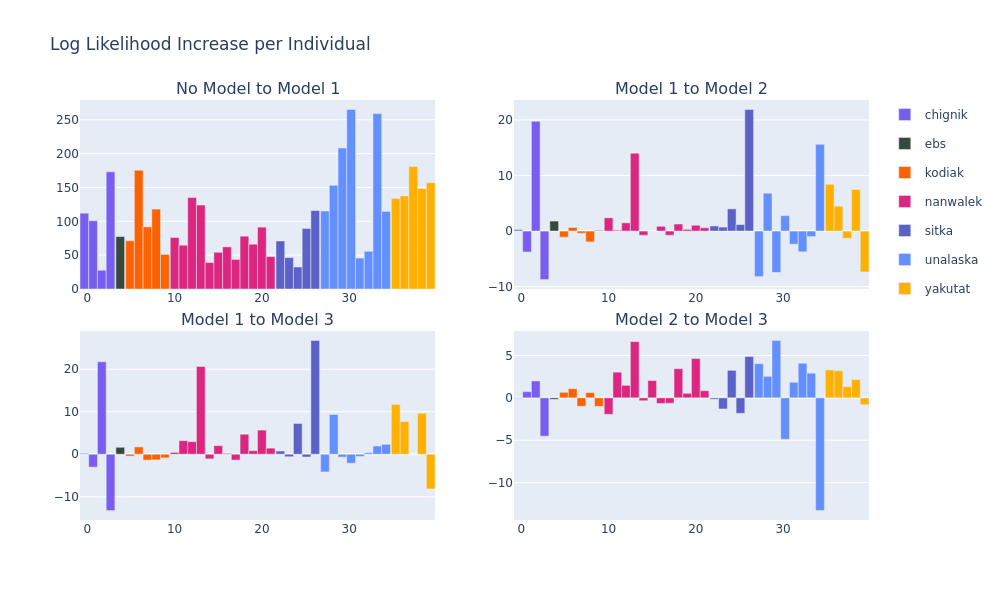
\includegraphics[height=70mm]{figures/ll_increase.png}
  \caption{Log likelihood increase (unnormalized) per individual of each model change.}
  \label{fig:ll_increase}
\end{figure}

\begin{figure}[h!] 
	\centering
  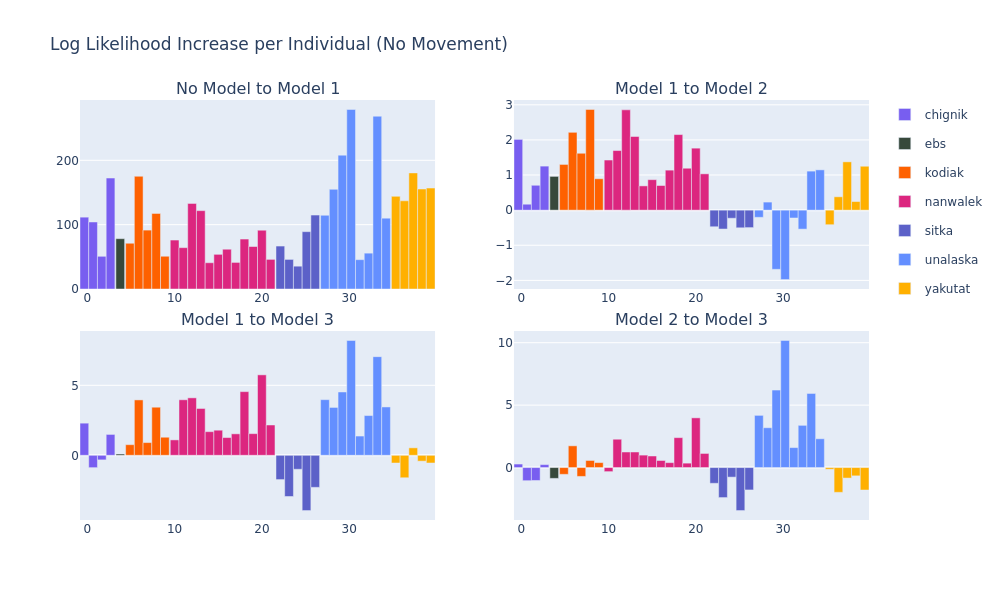
\includegraphics[height=70mm]{figures/ll_increase_no_movement.png}
  \caption{Log likelihood increase (unnormalized) per individual of each model change in cases where the selection involved no movement.}
  \label{fig:ll_increase_no_movement}
\end{figure}

\FloatBarrier

\begin{figure}[h!] 
	\centering
  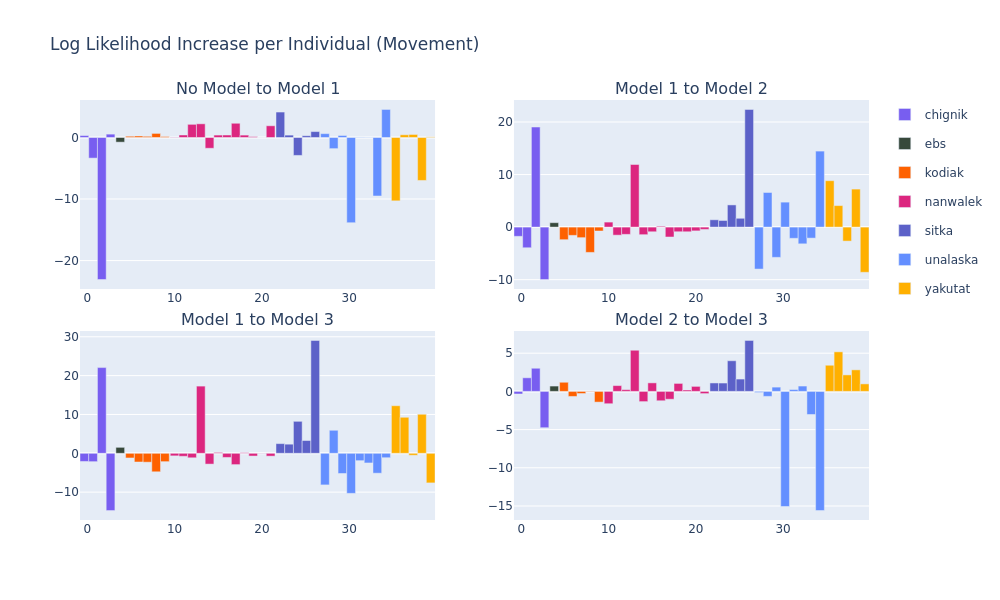
\includegraphics[height=70mm]{figures/ll_increase_movement.png}
  \caption{Log likelihood increase (unnormalized) per individual of each model change in cases where the selection involved movement.}
  \label{fig:ll_increase_movement}
\end{figure}



Figure \ref{fig:ll_increase} shows the unnormalized changes in log likelihood for each individual colored by the region in which they were initially tagged as we go from one model to the next. Figures \ref{fig:ll_increase_no_movement} and \ref{fig:ll_increase_movement} break this down for decisions that resulted in no movement and movement respectively. Only individuals in the validation set were considered.

The appendix contains a series of mapped examples (figures \ref{fig:chignik_map}-\ref{fig:yakutat_map}) from each of these regions (besides EBS) that shows how the log likelihood per decision (when moving) changed in moving from model 1 to model 2 and then from model 2 to model 3. As in the above, only individuals in the validation set were considered.\newline

Finally as much of the behavior seems to be modulated by movement distances (or lack of movement) a summary table of empirical likelihood of movement of a specific distance is given (taken over all individuals). 

\begin{center}
\begin{tabular}{| c | c | c |}
\hline
Distance Bin (km) & Likelihood of Selection & \# Training Decisions \\
\hline
No Movement & 65.6\% & 3163 \\
Up to 50km & 32.5\% & 1567 \\
50km to 100km & 1.9\% & 92 \\
\hline

\end{tabular}
\end{center}


\section*{Discussion}

\subsection*{Model One: Distance as a Key Feature}
Given the observations that most decisions involve an individual staying put (within its h3 cell) and rarely do fish travel to an h3 cell further than 50km away, it was decided that a more reasonable baseline model than even odds would be one that included distance traveled as a feature (model 1). 

As expected model 1 resulted in a significant improvement in log-likelihood across all individuals in the validation set as compared to a model that gives even odds to each available choice. This model therefore provides the baseline for our subsequent models. 

\subsection*{Model Two: Movement Heading}
Beyond this underlying distance feature, the interest is in predicting, when fish move, where they will move. Of particular interest was the individuals in the sitka and yakutat groups as these groups had several individuals exhibiting what appeared to be very directed and extensive movement. 

Upon studying these individuals it was noted that changes in mixed layer thickness seemed to incite movement and the individuals tended to stay (anecdotally) near higher primary productivity. Therefore a model with net primary productivity and mixed layer thickness was of interest. 

However, before moving to this model we wanted a baseline model that included movement heading as a feature so that we could determine what aspects of the movement were predicted simply by common headings as opposed to movement specifically related to productivity. Model 2 is this distance plus movement heading model. 

Looking at figure \ref{fig:ll_increase} we can see that for several individuals in the yakutat group adding movement heading increased the log likelihood meaningfully as compared to model 1 (our baseline). 
Indeed figure \ref{fig:ll_increase_movement} indicates that most of this increase comes from decisions where the individuals moved. Looking at figure \ref{fig:yakutat_map} it is clear that the move from model 1 to model 2 is creating a model that's learning a heading south east is more likely than alternative directions with the movements of fish in north or westerly directions actually reducing in log likelihood as compared to the baseline. 

This southeasterly pattern is maintained throughout figures \ref{fig:chignik_map}-\ref{fig:yakutat_map} and indeed looking at \ref{fig:ll_increase_movement} there are several groups where the majority of individuals suffer a decrease in log likelihood, in all likelihood due to this common direction not being representative of them.  

The sitka group however does see an improvement as well showing that both of these majority south eastern movement groups (sitka and yakutat) can be at least partially explained by a common heading down the coast. 

\subsection*{Model Three: Environmental Features}
With this naive heading baseline in place we can now investigate the extent to which adding in net primary productivity and mixed layer thickness allows our model to distinguish when different headings are taken by different fish, or in fact reinforce the headings already "selected". 

Looking at the step from model 2 to model 3 in figures \ref{fig:chignik_map}-\ref{fig:yakutat_map} we see now that several of the movements that saw a drop in log likelihood as compared to the model 1 baseline are actually seeing a rise in log-likelihood under this new model indicating that the new features are allowing us to swing the preferred movement heading in a way that is conditioned on the environment. 

In addition, especially in the sitka group, we see reinforcement/refinement of the decisions as there is an increase in log likelihood up and beyond what was received from model 2. That is to say that while there is a general tendency in the south easterly direction, the specific cells chosen are in some way correlated to productivity. 

Noteable as well is the fact that the move from model 2 to model 3 had a significant positive impact on the predictability of the decisions from the nanwalek group, much more so than in the step from model 1 to model 2. The kodiak group however remains largely unaffected. 

\subsection*{Further Questions}

Looking at the cases in figure \ref{fig:ll_increase} in which we see significant drops in log likelihood or cases where there is no meaningful change we can see that while there is predictive power in the features chosen thus far - especially for the yakutat, sitka, and nanwalek groups - there are still plenty of individuals that can act as exemplars for searching for new behavioral drivers. 

For example in figure \ref{fig:chignik_map}, even with the addition of the productivity features in model 3 the westerly movements are still poorly predicted and would warrant investigation. 

Likewise the unalaska group is poorly explained in general and would represent another case study for further investigation. Perhaps by training a model with the same set of features as model 3 but only over this group we would see a significant improvement in the performance of the model which may lead us to look for demographic or geophysical differences that could explain how two different groups of fish are "using" the same covariates so differently. 

All in all though, the models we have allow us to identify and focus upon individuals that so far resist our attempts to explain them. 

\subsection*{Conclusion}

This investigation demonstrates the power and flexibility of an iterative modeling approach for modeling behavior. By building baseline models and progressively refining them with additional covariates, we identify both predictive patterns and individuals resistant to explanation, which serve as focal points for further hypothesis generation. The efficiency of this process, enabled by quick training times and parallelization, ensures that refinement is limited only by the investigator's ability to propose and test new hypotheses. Crucially, at every stage, the models not only advance understanding but remain actionable for predictions, underscoring their dual utility as tools for both discovery and application. 

\newpage

\section*{Code}

The tooling used to build these models as well as the means to deploy them using Amazon Web Services has been packaged at: \newline https://github.com/networkearth/mimic

\bibliographystyle{apalike}
\bibliography{reference}
\newpage
\section*{Appendix: Mapped Examples}

\begin{figure}[h!] 
	\centering
  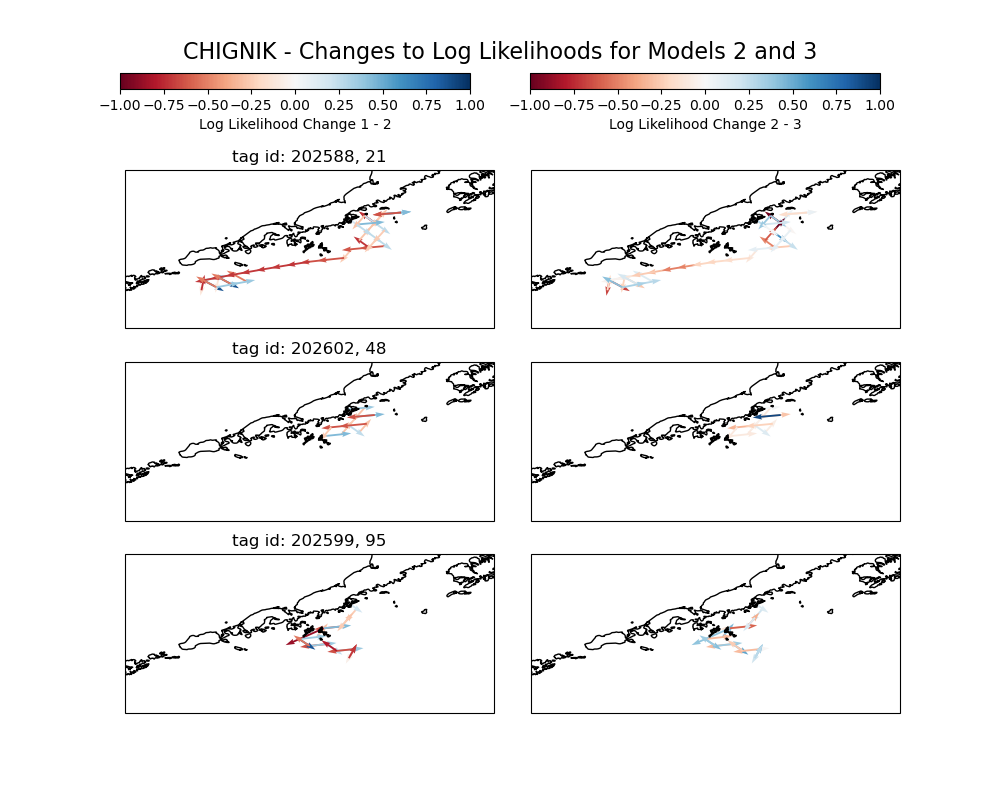
\includegraphics[width=140mm]{figures/chignik_map.png}
  \caption{Log likehood changes per decision - Chignik}
  \label{fig:chignik_map}
\end{figure}

\begin{figure}[h!] 
	\centering
  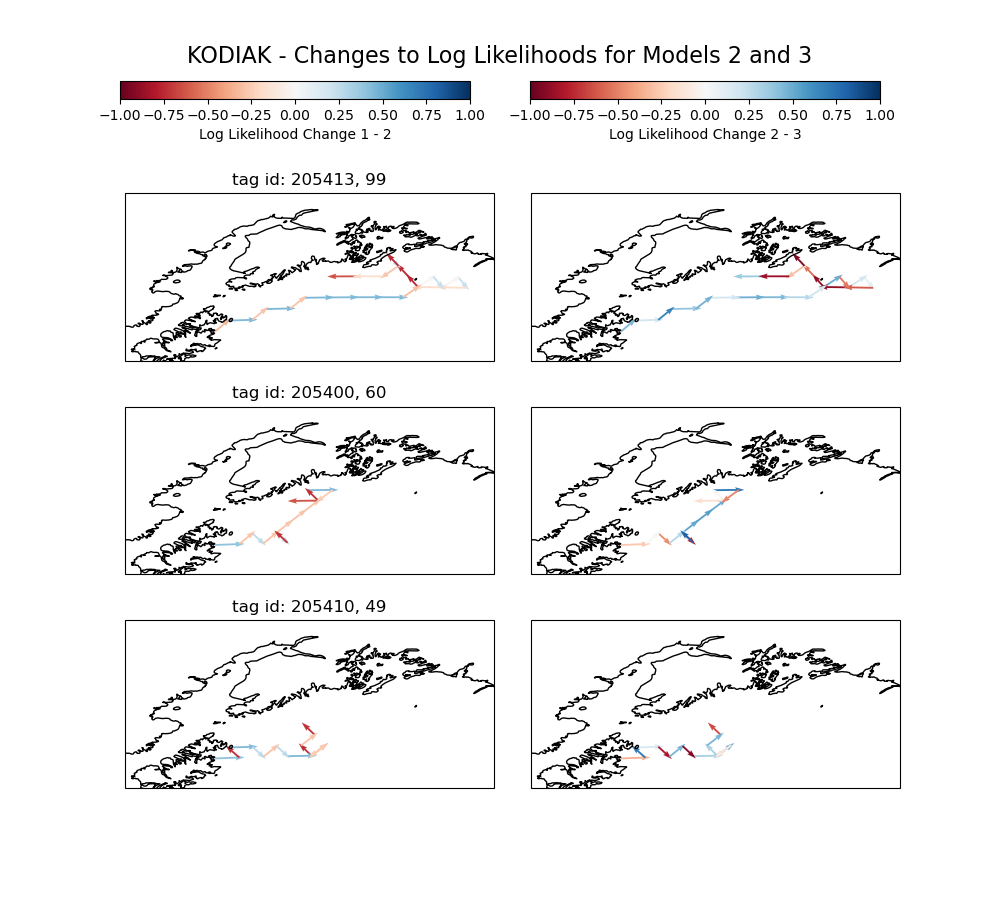
\includegraphics[width=140mm]{figures/kodiak_map.png}
  \caption{Log likehood changes per decision - Kodiak}
  \label{fig:kodiak_map}
\end{figure}

\begin{figure}[h!] 
	\centering
  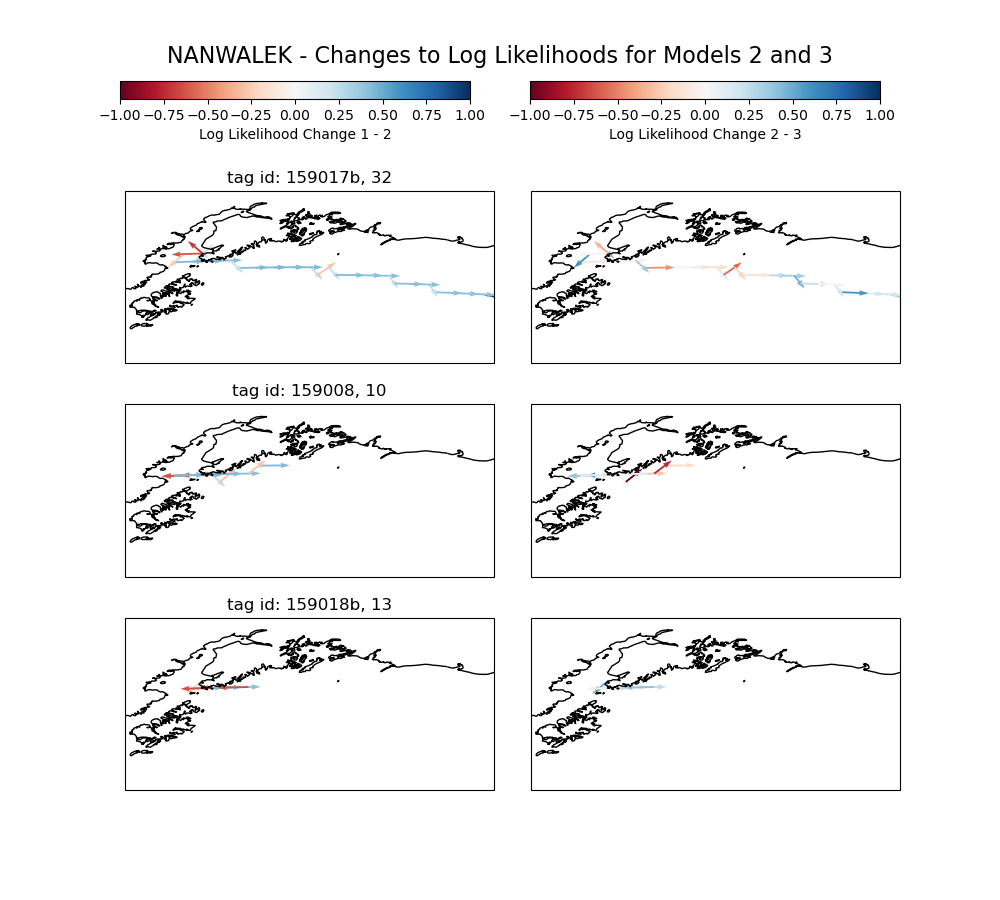
\includegraphics[width=140mm]{figures/nanwalek_map.png}
  \caption{Log likehood changes per decision - Nanwalek}
  \label{fig:nanwalek_map}
\end{figure}

\begin{figure}[h!] 
	\centering
  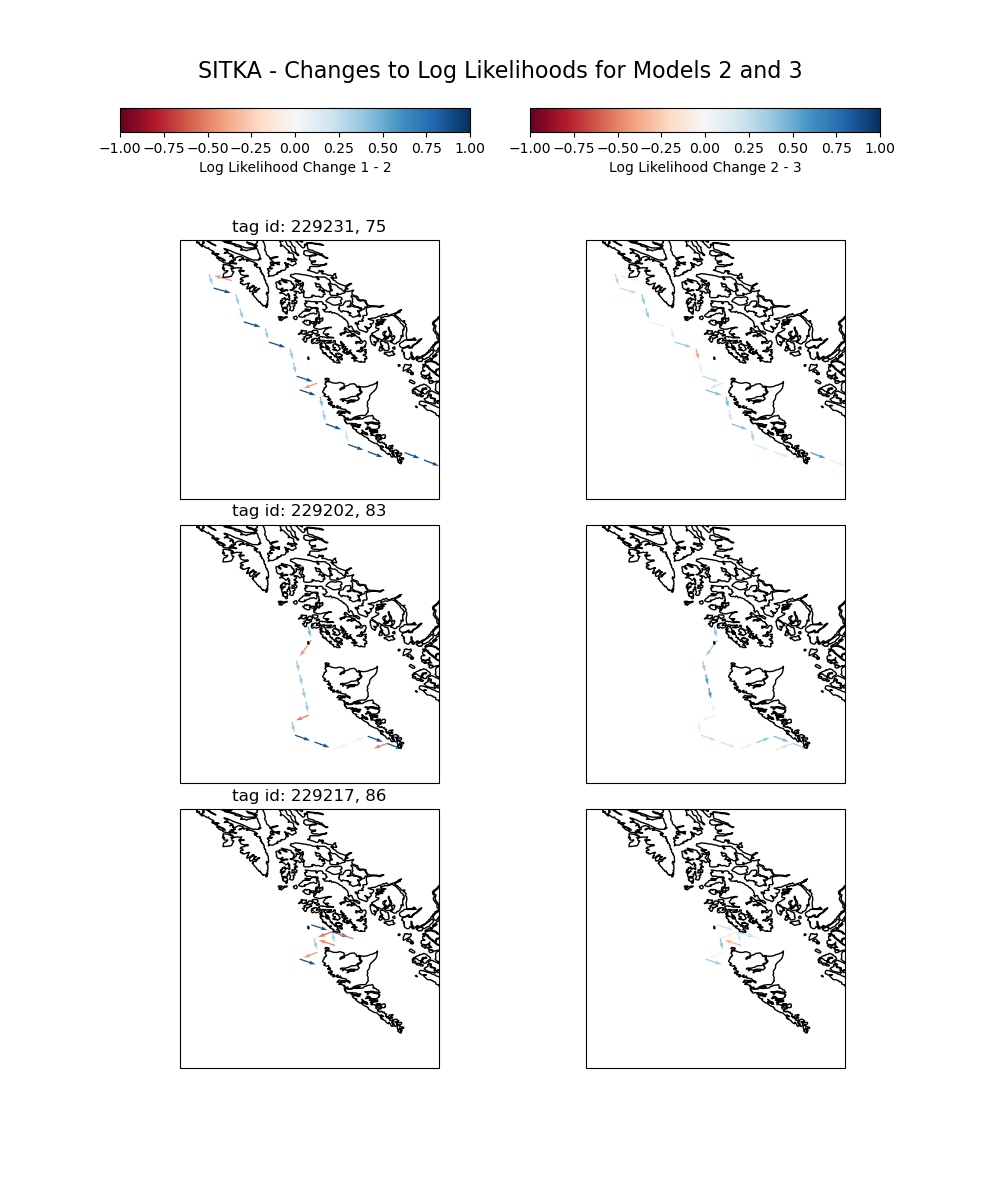
\includegraphics[width=140mm]{figures/sitka_map.png}
  \caption{Log likehood changes per decision - Sitka}
  \label{fig:sitka_map}
\end{figure}

\begin{figure}[h!] 
	\centering
  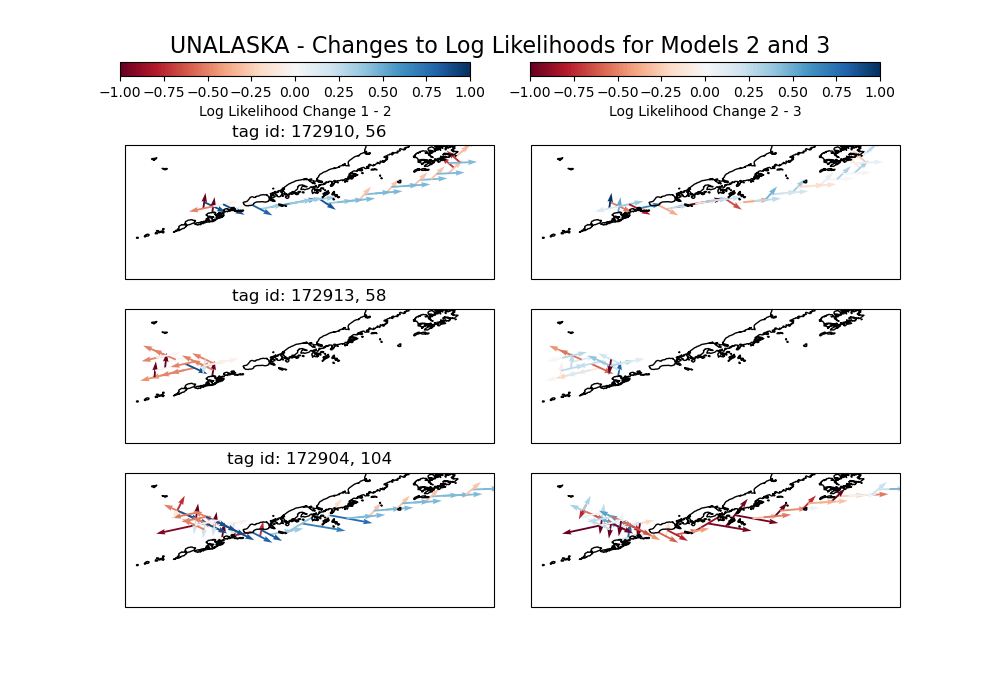
\includegraphics[width=140mm]{figures/unalaska_map.png}
  \caption{Log likehood changes per decision - Unalaska}
  \label{fig:unalaska_map}
\end{figure}

\begin{figure}[h!] 
	\centering
  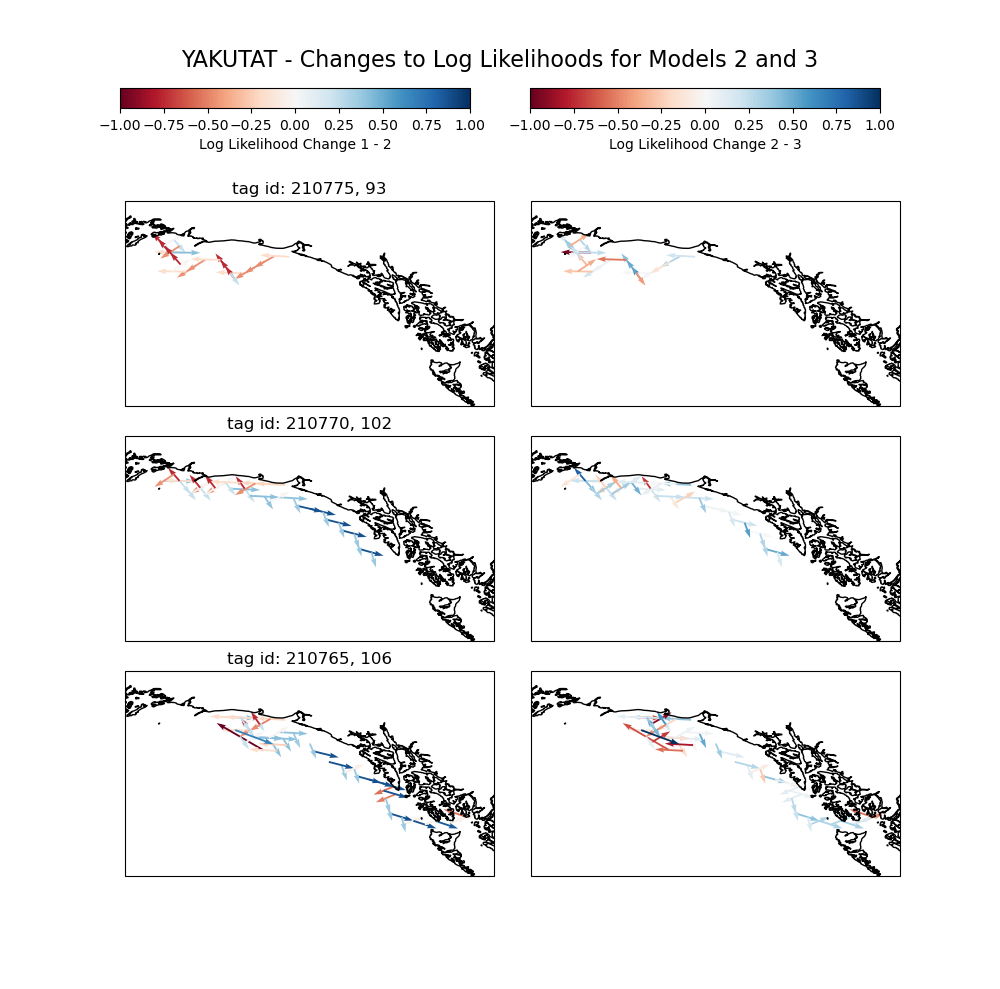
\includegraphics[width=140mm]{figures/yakutat_map.png}
  \caption{Log likehood changes per decision - Yakutat}
  \label{fig:yakutat_map}
\end{figure}

\end{document}